\section{Progettazione}

\subsection{Database}
L'analisi dei requisiti ha portato alla definizione di uno diagramma Entità-Relazione normalizzato per definire una Base di Dati
che gestisse utenti, ristoranti, recensioni e preferiti.
\begin{figure}[H]
  \centering
  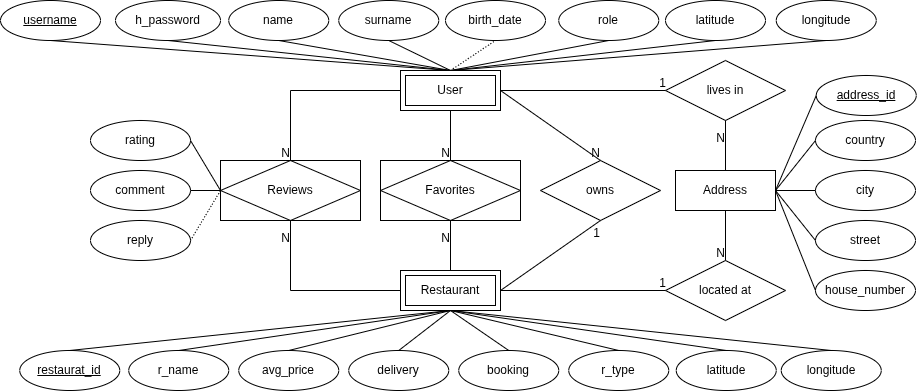
\includegraphics[width=\textwidth]{images/ER-refactored.png}
  \caption{Diagramma ER}
  \label{fig:er-diagram}
\end{figure}

\subsection{Use-Case Diagram}
Per ciascuna tipologia di utente (ospite, cliente, ristoratore) sono stati individuati 
i casi d'uso principali, dalla ricerca di ristoranti alla gestione 
di recensioni e risposte.

\begin{figure}[H]
  \centering
  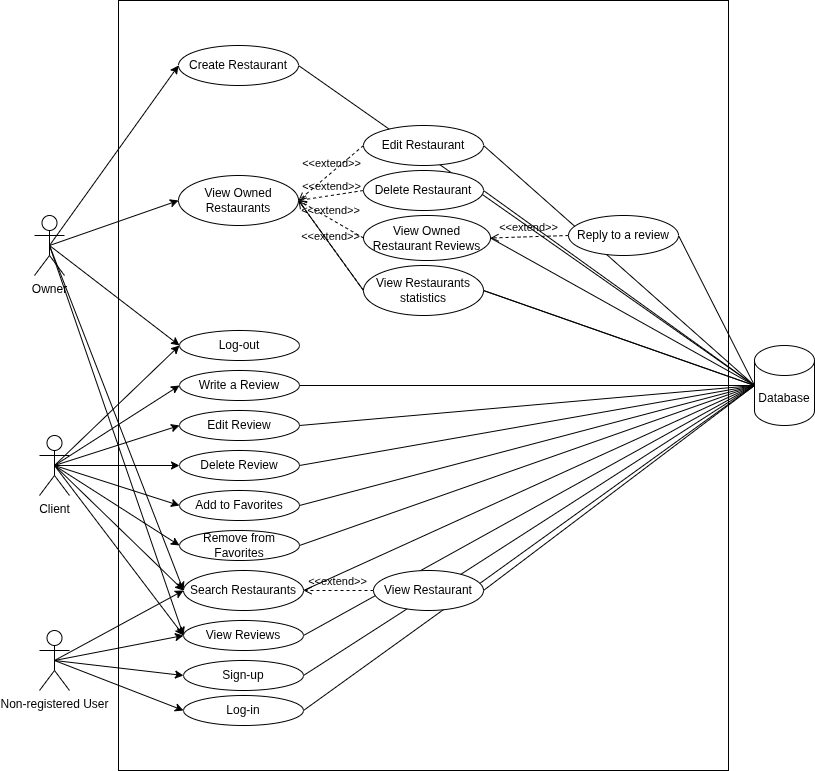
\includegraphics[width=\textwidth]{images/UML-Use-Case.png}
  \caption{User-Case Diagram}
  \label{fig:usecase-diagram}
\end{figure}
